\begin{figure*}[ht!]
\centering
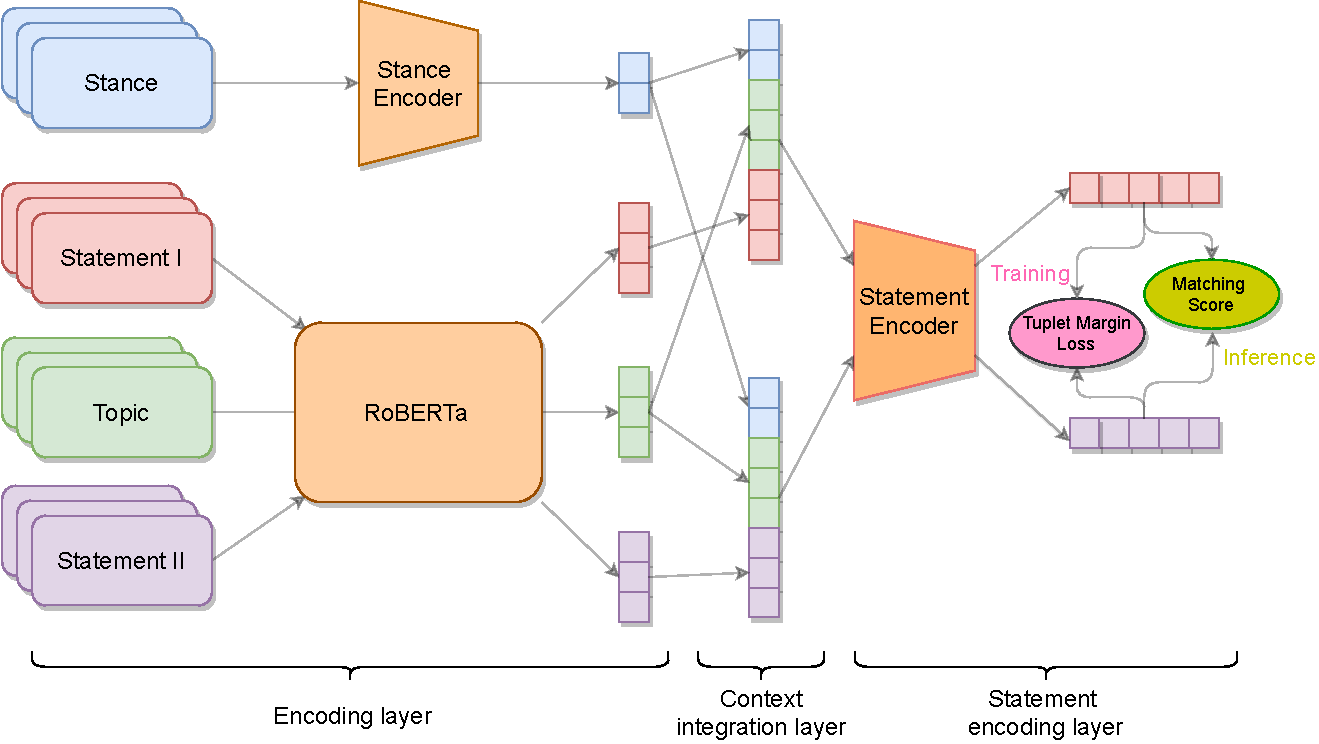
\includegraphics[scale=0.6]{figures/KPA-model.pdf}
\caption{The overall design of our Matching The Statements architecture.}
\label{fig:model}
\end{figure*}

\section{Related Work}
\label{sec:related-work}
A standard approach for key points and arguments analysis is properly extracting their meaningful semantics. Our model stems from recent literatures that are based on siamese neural networks \citep{reimers-gurevych-2019-sentence, gao2021simcse} to measure the semantic similarity between documents. Even though, MTS has its own unique characteristics to incorporate context information.
\subsection{Sentence Embeddings} 
The representation of sentences in a fixed-dimensional vector space plays a crucial role in enhancing a model's performance on downstream tasks. Early methods relied on static word embeddings \citep{pennington-etal-2014-glove, bojanowski2017enriching}, which encoded a sentence by directly averaging its word vectors or employing recurrent neural network (RNN) encoders \citep{conneau-etal-2017-supervised} and taking the pooled output from the hidden units. Despite the fact that these methods can leverage both syntactic and semantic features, they often fail to retain the contextual information or suffer from slow training (due to the sequential nature of RNNs). 

That is where BERT \cite{devlin2018bert} as well as its variants come in and dominate the modern NLP research. Training these architectures can exploit the parallel computational capacity of GPUs/TPUs hardware accelerators. In SBERT, \citet{reimers-gurevych-2019-sentence} proposed a sentence embedding method via fine-tuning BERT models on natural language inference (NLI) datasets. More recent studies in learning sentence representation followed the contrastive learning paradigm and achieved state-of-the-art performance on numerous of benchmark tasks \citep{liao2021sentence, yan2021consert}.

\subsection{Semantic matching} 

Semantic matching is a long-standing problem and has a wide range of applications, such as: question-answering \citep{yang-etal-2015-wikiqa}, text summarization \citep{zhong-etal-2020-extractive} and especially, information retrieval \citep{huang2013learning, guo2016deep}. \citet{jiang2019semantic} introduced a hierarchical recurrent neural network that could capture long-term dependency and synthesize information from different granularities (i.e. words, sentences or paragraphs). Similarly, \citet{yang2020beyond} replaced the RNN backbones with transformer-based models and modified self-attention architectures to adapt with long document inputs. 

However, most of the existing work focuses only on assessing the similarity between pairs of sentences without paying attention to their context - which can help the reader to get an overview of the discussed topic. Recently, the ArgKP-2021 dataset has been published by \citet{bar-haim-etal-2020-arguments}, which consists of annotations about whether two statements and their stances towards a specific topic match or not. The next sections will provide an overview of this dataset and how our model is applicable in the Quantitative Summarization – Key Point Analysis Shared Task \footnote{\url{https://2021.argmining.org/shared_task_ibm.html}}.